\chapter{Solution}
In this chapter the CloudASR implementation will be described.
The implementation was affected by three key requirements:

\begin{itemize}
  \item
    \textbf{Scalability} -
      because the speech recognition is a demanding process in terms of computational resources,
        it is not possible to handle many parallel requests on one machine.
      Therefore the CloudASR architecture is designed to be able to scale across many machines.

  \item
    \textbf{Customizability} -
       there are already several webservices that provide an API for speech recognition,
         but they are not easily customizable.
       Thus, the second requirement was to be able to host any Kaldi model on  the CloudASR platform.
       Moreover, the CloudASR platform is able to run any ASR system,
         if the users implement a wrapper for that system.

  \item
    \textbf{Easy deployment} -
      complex systems as CloudASR have many dependencies and a difficult deployment process,
        which makes their maintenance hard.
      CloudASR is designed to has as few dependencies as possible and an one command deployment.

\end{itemize}

\IDEA{Mention somehow Batch/Online recognition mode}


\section{Architecture}
In order to meet the aforementioned scalability requirement
  the platform had to be designed from the very beginning to be able to run on many machines.
To be able to do that the architecture consits of several nodes
  that communicate with each other by sending messages over ZeroMQ sockets
  (each node acts as an actor as described in \cite{hewitt1977viewing}).
Another problem is that it is not possible start to an ASR system when the user sends a request,
  because the ASR systems need some time load decoding graphs in memory
  and this would add some unnecessary latency.
Therefore the platform uses Master-Worker architecture to be able to handle many parallel requests for various languages.

The CloudASR architecture as described in Figure~\ref{fig:architecture} consists of several types of nodes that can run on different machines.
These nodes are \textbf{Master}, \textbf{Worker}, \textbf{API}, \textbf{Web},  and \textbf{Recordings Saver}.
In the following section each node will be described in detail.


\begin{figure}[h]
  \centering
  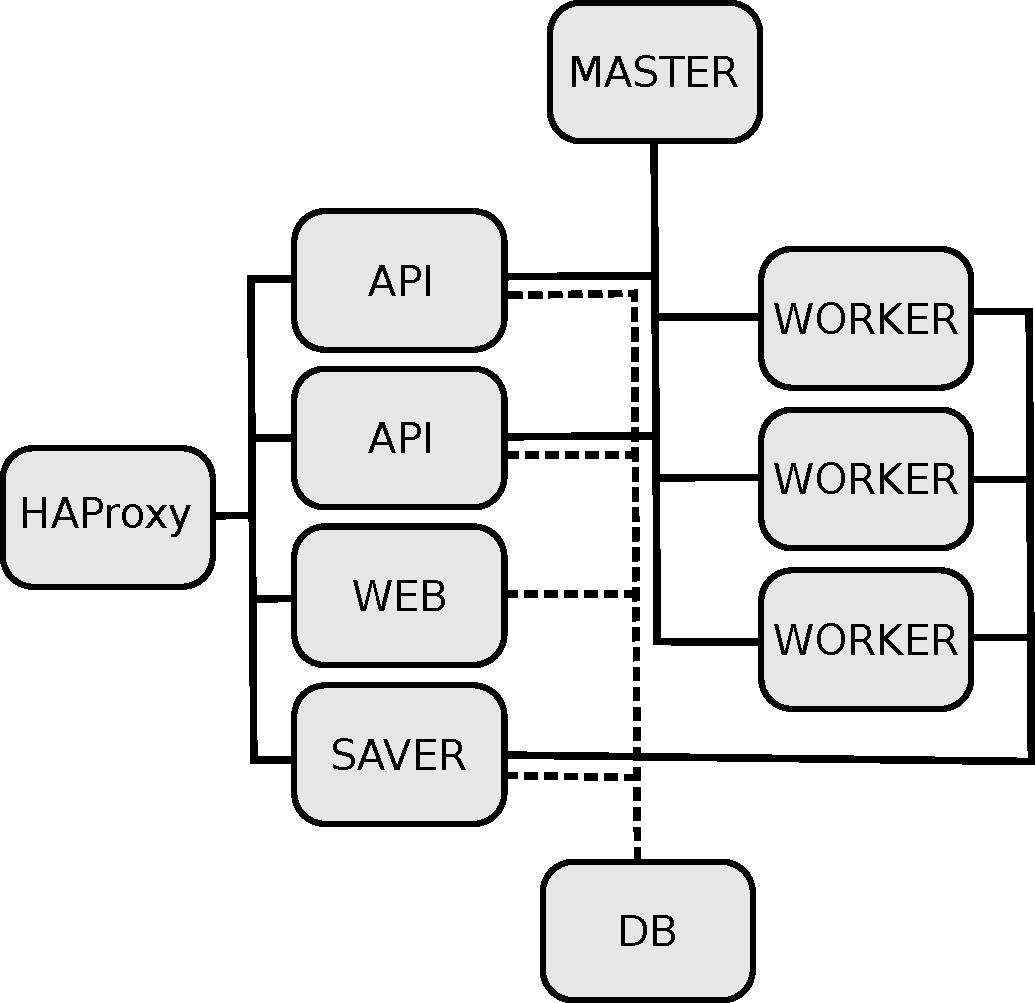
\includegraphics[width=0.75\textwidth]{./img/architecture.pdf}

  \caption{
    An overview of the CloudASR architecture.
    The most important node is \textbf{Master} to which \textbf{Workers} sends heartbeats with their state.
    The client requests are handled by \textbf{API} which communicates with Master and Workers.
    The processed recordings are sent to \textbf{Saver} which saves them and serves them via HTTP.
    An annotation interface and an online demo are hosted by \textbf{Web}.
    Finally, there are also two externals nodes \textbf{HAProxy}
      which load-balances requests between particular application instances
      and \textbf{DB} which stores information about processed recordings.
  }
  \label{fig:architecture}
\end{figure}


\subsection{Master}
The main task of Master is to keep track about running workers and scheduling tasks to them.
In order to be able to handle requests for various languages
  Master has a queue of waiting workers for each language.
Running workers send heartbeats, small messages with information about their state, to Master
  and when the Api asks for a worker Master can return address of an available worker.
This makes it possible to dynamically add/remove new workers without need to restart the CloudASR platform.

The workers can be in four different states:
  \textbf{started}, \textbf{waiting}, \textbf{working} and \textbf{not responding}
  and they send four different heartbeats:
  \textbf{started}, \textbf{waiting}, \textbf{working} and \textbf{finished}.

The lifecycle of the worker as described in Figure~\ref{fig:worker-state} starts in in the \textbf{started} state,
  after that it moves to the \textbf{waiting} state by sending the \textbf{waiting} heartbeat.
The worker remains in the waiting state until \textbf{Master assings a tasks} to it,
  then it moves to the \textbf{working} state
  where it remains as long as it is working.
In the working state worker sends working heartbeats periodically,
  to inform Master that it is working and it did not fail.
At the end of the task the Worker sends \textbf{finished} heartbeat
  and Master changes the state of the Worker to the \textbf{waiting} state.

Additionally, when a worker crashes during the processing of the task and it gets restarted,
  it sends started heartbeat again,
  which informs Master, that the worker was restarted and it adds it to the queue again.
When a worker does not send any heartbeat for 10 seconds,
  the master set the worker state to \textbf{not responding}.
But as soon as the worker sends any heartbeat,
  the master will set the worker to the appropriate state.

\begin{figure}[h]
  \centering
  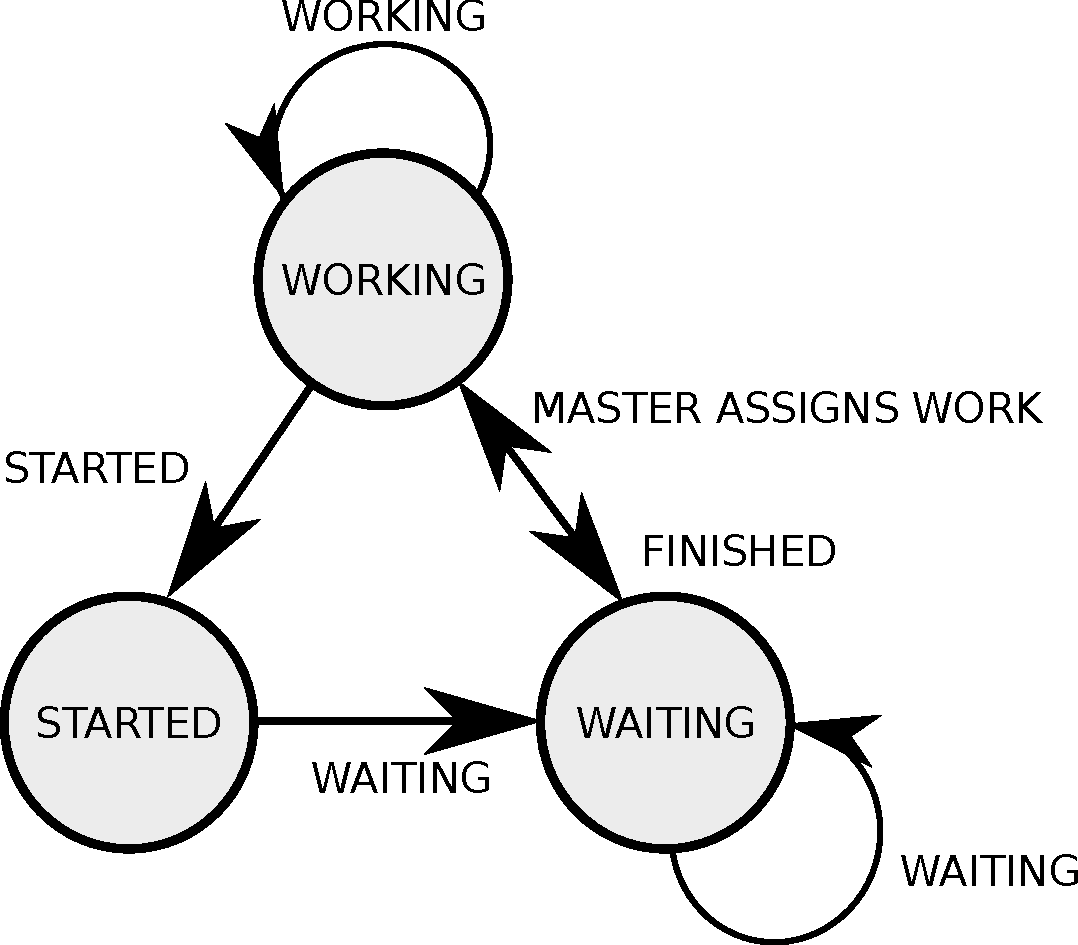
\includegraphics[width=0.75\textwidth]{./img/worker-state.pdf}

  \caption{
    The lifecycle of the worker starts in in the \textbf{started} state,
      after that it moves to the \textbf{waiting} state by sending the \textbf{waiting} heartbeat.
    The worker remains in the waiting state until \textbf{Master assings a tasks} to it,
      then it moves to the \textbf{working} state
      where it remains as long as it is working.
    In the working state worker sends working heartbeats periodically,
      to inform Master that it is working and it did not fail.
    At the end of the task the Worker sends \textbf{finished} heartbeat
      and Master changes the state of the Worker to the \textbf{waiting} state.
  }
  \label{fig:worker-state}
\end{figure}

Unfortunately, Master is a single point of failure of the CloudASR platform.
When Master stops working no speech recognition requests can be processed,
  because the API containers will not know to which worker they can forward the request.
But as soon as Master starts working the platform should be available again.


\subsection{Worker}
Worker is a wrapper for an ASR system.
By default Pykaldi is used but any other ASR system can be used
  if the users implement a python wrapper for that system.
Because CloudASR should be able to process very long recordings in the online mode,
  it is neccessary to split the recordings into smaller chunks
  that can be processed with limited computational resources.
For that purpose VAD component from Alex Statistical Dialogue Systems Framework \cite{jurcicek2014alex} is used to detect silence in a speech,
  because the speech can be splitted at that point without any large negative effect on the accuracy of the transcriptions.

\IDEA{
  At the end of the recognition Worker sends the whole recording together with respective n-best list to Saver.
  Heartbeats
    that Worker sends to Master
    are small messages with Worker address, language it processes and its state.
}


\subsubsection{Deployment of New Kaldi Worker}
One of the key requirements for CloudASR was customizability,
  primarily customizability of the workers decoding graphs.
Therefore, CloudASR supports an easy way for users to add their own Kaldi models.
The only thing that the users have to do is to create a worker docker image with their models.

The creation of a worker docker image consists of several steps.
First, users have to create a script \texttt{download\_models.sh} which will download all necessary files from their server,
  see Figure~\ref{fig:download-models} for example.
Second, they have to create a configuration file \texttt{config.py} with appropriate configuration for the downloaded models,
  see Figure~\ref{fig:config-py}.
Finally, they have to copy a Dockerfile (see Figure~\ref{fig:worker-dockerfile}for example) for the worker
  and build the docker image with the appropriate command.
After that users can use the new worker in their application in the similar way as they use other models.

It is important to note that the new worker docker image will be available only on the machine where it was built.
If the users want to use this model on multiple machines, they have to push to their docker registry
  or alternatively they can update Jenkins scripts \texttt{build\_workers.sh} and \texttt{push\_workers.sh} to do that for them.

\begin{figure}[h]
  \verbatiminput{snippets/download_models.sh}

  \caption{An example of download\_models.sh script.}
  \label{fig:download-models}
\end{figure}

\begin{figure}[h]
  \verbatiminput{snippets/config.py}

  \caption{An example of config.py script.}
  \label{fig:config-py}
\end{figure}

\begin{figure}[h]
  \verbatiminput{snippets/Dockerfile_cs_alex}

  \caption{An example of worker Dockerfile.}
  \label{fig:worker-dockerfile}
\end{figure}


\subsubsection{Deployment of Arbitrary Worker}
Even though CloudASR supports only Kaldi out of the box, other ASR systems can be used too.
Again, the only thing that the users has to do is to create a worker docker image with their ASR system.
The only step that differs from the previous process is
  that the users have to implement and add to the Dockerfile a script \texttt{asr.py} with their own \texttt{create\_asr} method
  that returns \texttt{ASR} class with these methods:

\begin{itemize}
  \item
    \texttt{reset()} - this method is called after every requests
      and it can be used to reset the underlying ASR system.

  \item
    \texttt{recognize\_chunk(pcm)} - this method is used to process small chunks of recordings.
      The method should accept pcm chunks with frame rate 16000
        and it should return an interim hypothesis in form of a tuple \texttt{(confidence, transcript)}.

  \item
    \texttt{get\_final\_hypothesis} - this method is called at the end of every requests,
      it should return a list of n-best hypotheses in form of a tuple \texttt{(confidence, transcript)}.

\end{itemize}


The creation of such a script is illustrated on Figure~\ref{fig:dummyasr} on the DummyASR class,
  which will be also used for benchmark purposes in the Chapter~\ref{chapter:evaluation}.

\begin{figure}[h]
  \verbatiminput{snippets/dummy_asr.py}

  \caption{An example of alternative ASR implementation.}
  \label{fig:dummyasr}
\end{figure}


\subsection{API}
The main task of the API container is to forward requests from the clients to the workers.
The requests are either in form of HTTP POST for the batch mode or Socket.IO for the online mode.
The API is built on top of Flask framework with enabled asynchronous processing
  which allows single API container to process many parallel requests,
  because there are no blocking operations in the API container -
  it just receives requests from clients and forwards them via ZeroMQ to the workers.


\subsection{Web}
CloudASR platform has a web interface with an online demo and an annotation interface.
The online demo (See Figure~\ref{fig:webdemo}) allows users to try out CloudASR directly in their web browsers.
It has two modes, namely, dictation mode that only shows the best transcription of the recording
  and evaluation mode that also allows users to confirm that the transcription of the recording is correct.

\begin{figure}[h]
  \centering
  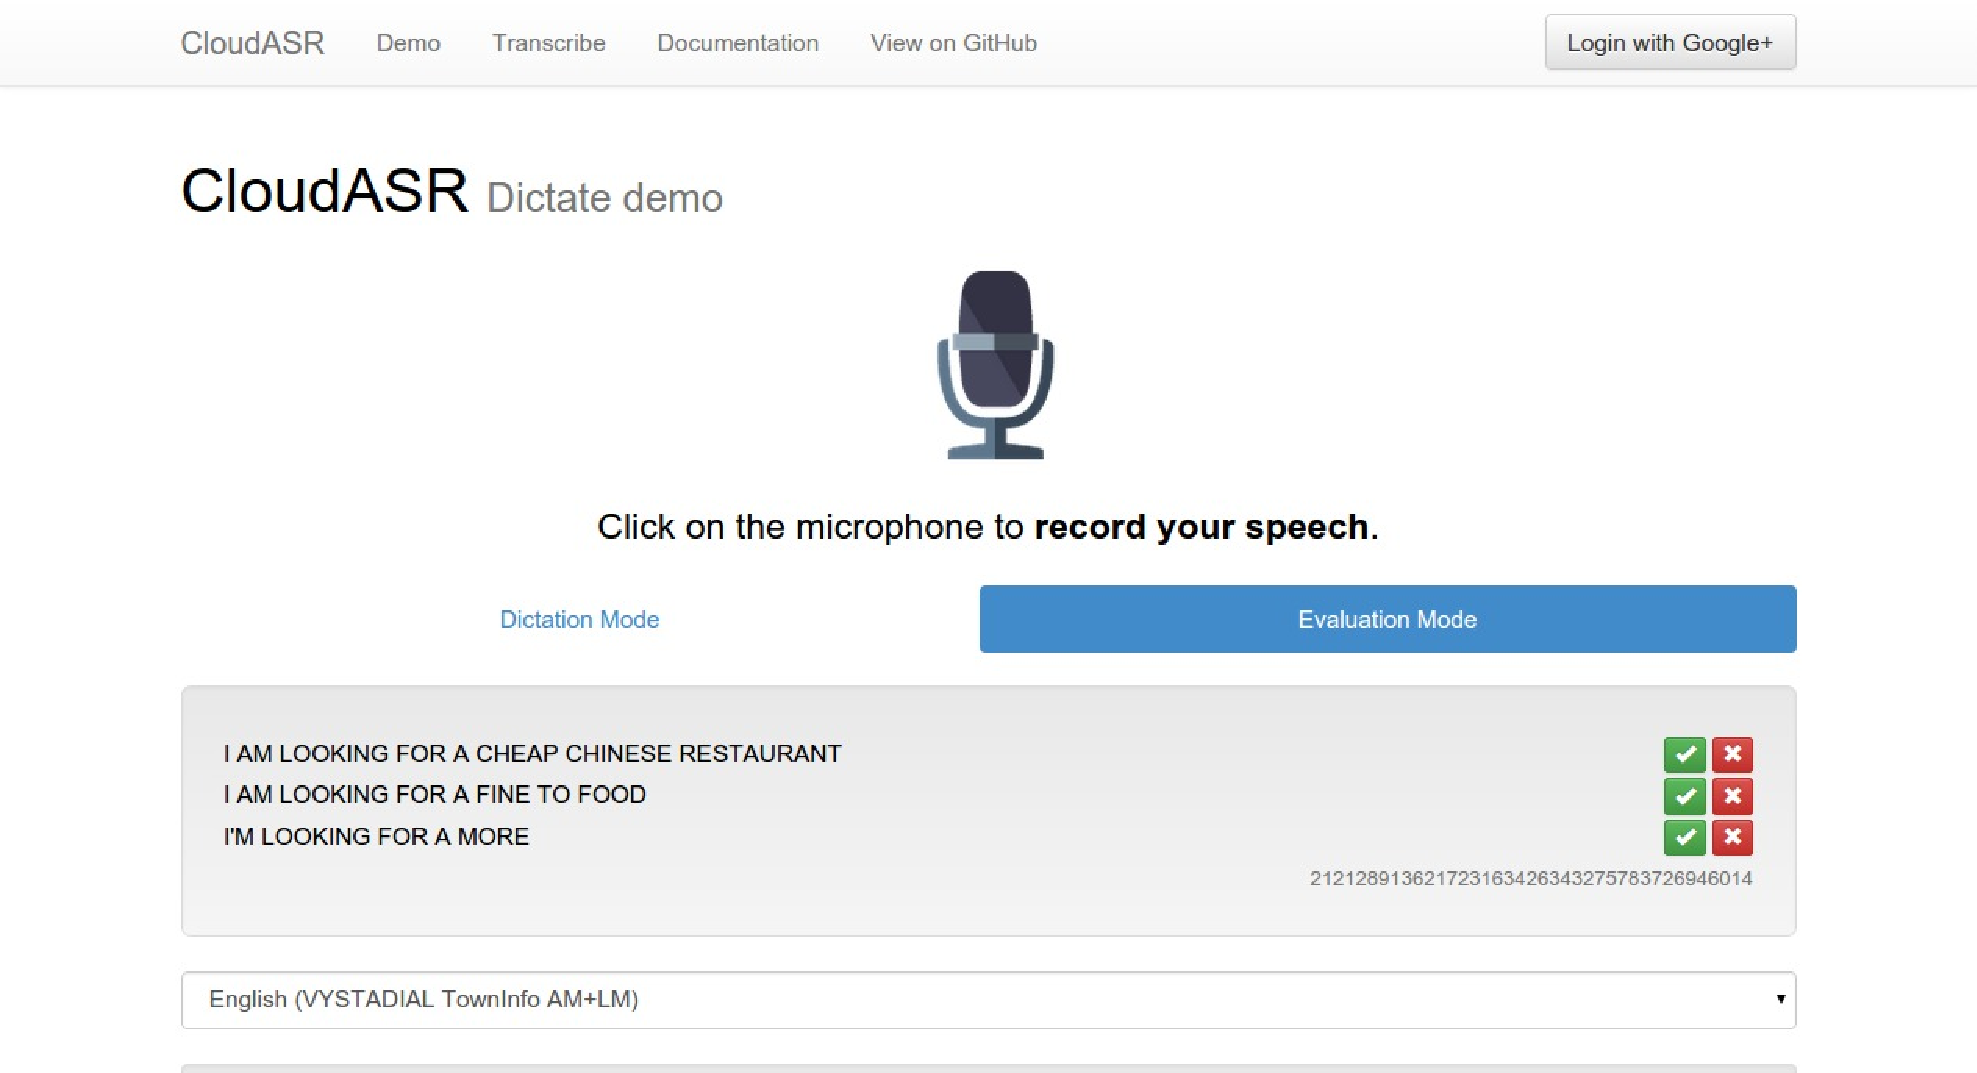
\includegraphics[width=0.95\textwidth]{./img/demo.pdf}

  \caption{Screen of the Web Demo}
  \label{fig:webdemo}
\end{figure}

The annotation interface distinguishes between two types of user roles: users and administrators.
Normal users are only allowed to add transcriptions (See Figure~\ref{fig:annotation-interface}) to the recordings.
Administrators can also browse all recordings with their transcriptions and manage workers descriptions.

\begin{figure}[h]
  \centering
  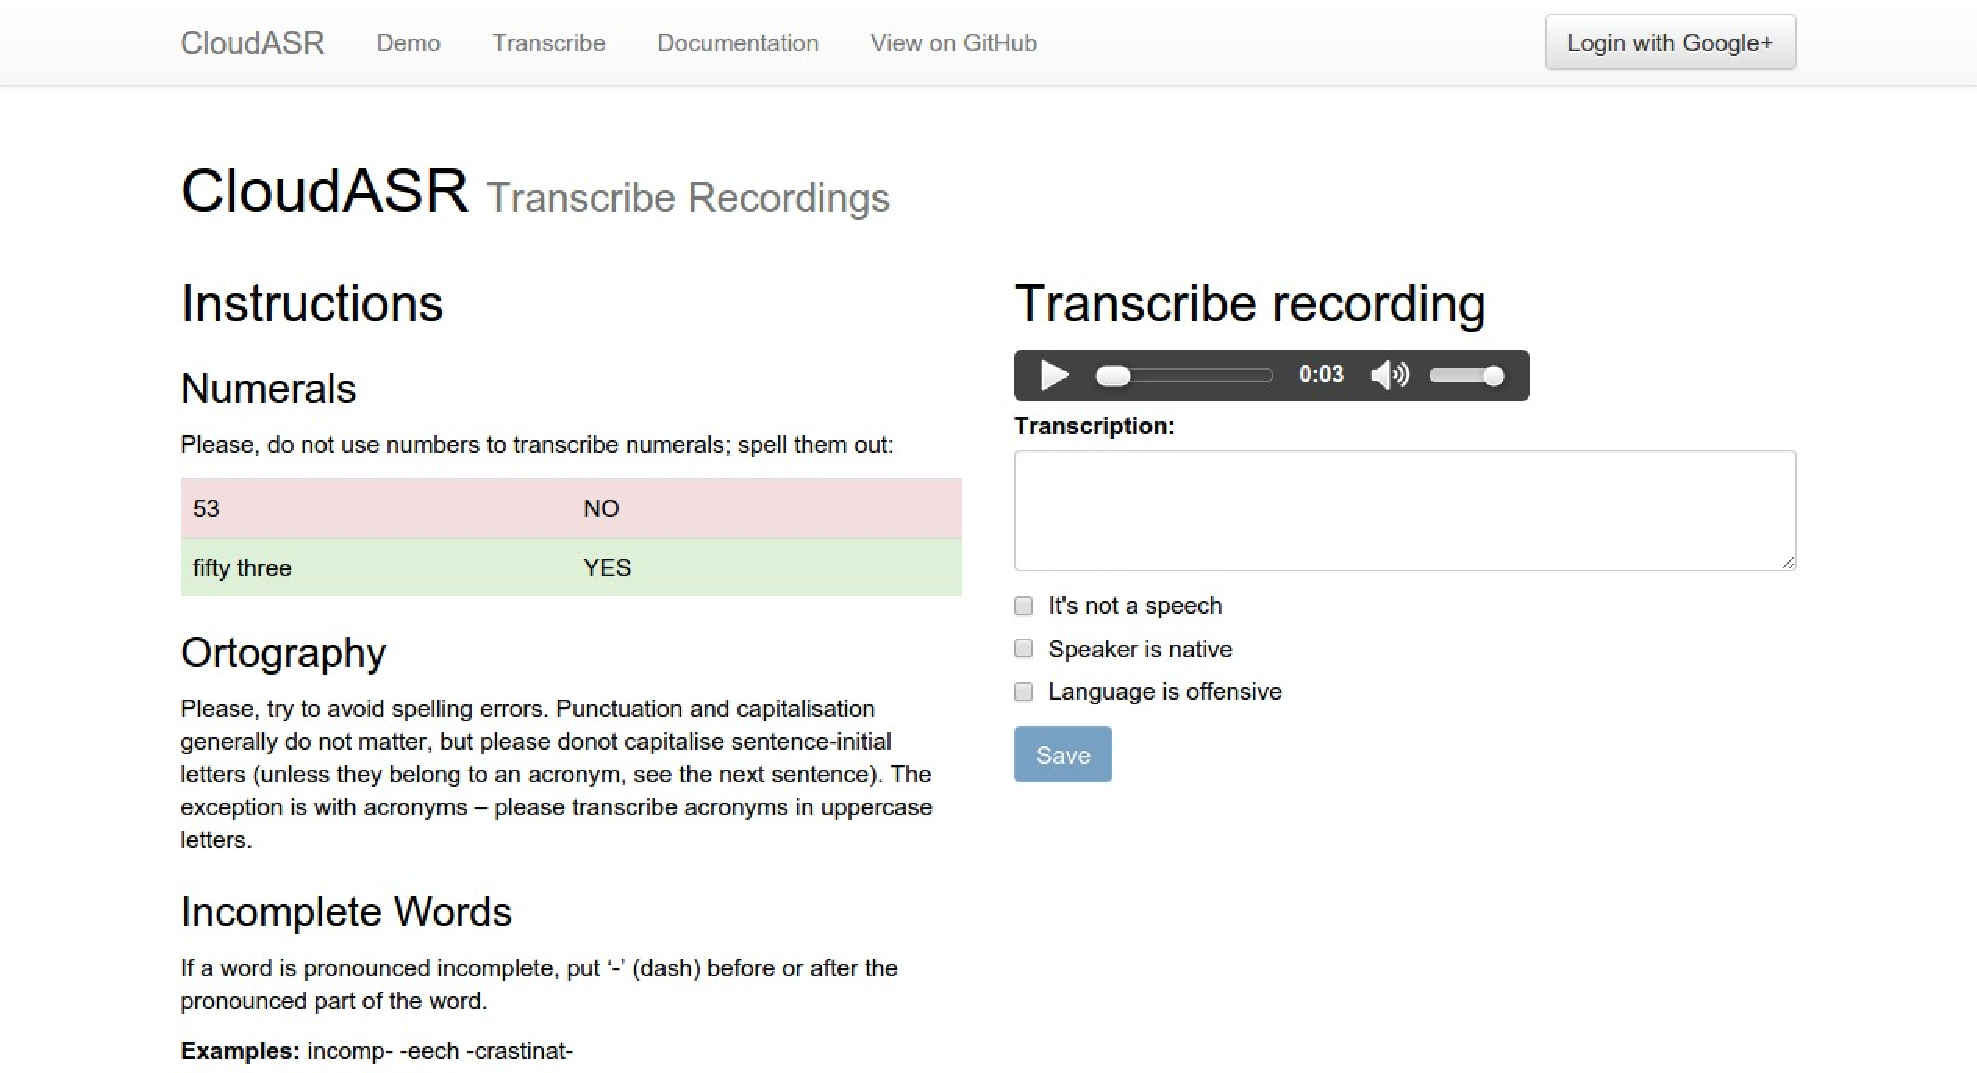
\includegraphics[width=0.95\textwidth]{./img/annotation.pdf}

  \caption{Screen of the Annotation Interface}
  \label{fig:annotation-interface}
\end{figure}

\IDEA{mention google+ login}
\IDEA{Describe process of annotation}
\TODO{Think of ROVER to merge user transcriptions.}



\subsection{Recordings saver}
The main task of the Recordings saver is to save and serve recordings processed by workers.
When the worker finishes recognition it sends the recording with its n-best hypotheses to the Recording saver via ZeroMQ socket.
The saver saves the wave file to the filesystem and it save the n-best hypotheses to the database so that they can be used in the future.

\TODOIMG{fig:db-schema}{Database schema}


\section{Request Workflow}
The CloudASR platform supports both batch and online speech recogntion.
In the batch mode users sends wave files to the API using HTTP POST request
  and they receive a json with a n-best transcriptions.
Users can specify which worker they want to use in \texttt{lang} parameter.
The batch mode has a similiar interface to Google Speech API,
  which enables users to switch to CloudASR seamlessly.
An example of batch recognition API usage is illustrated on a simple curl command in Figure~\ref{fig:curl},
  a response from the API is shown in Figure~\ref{fig:curl-response}.

\begin{figure}[h]
  \verbatiminput{snippets/curl.bash}

  \caption{An example of batch speech recognition mode request for an en-towninfo worker using curl.}
  \label{fig:curl}
\end{figure}

\begin{figure}[h]
  \verbatiminput{snippets/curl.json}

  \caption{An example response of batch recognition mode.}
  \label{fig:curl-response}
\end{figure}

In contrast to batch mode in online mode users sends PCM chunks of a recording while the recording is recorder.
Users can send these chunks as often as they want
  but it is advised to send a chunk four times per second
  to achieve a smooth experience.
Chunks are sent to the server via Socket.IO technology encoded as a JSON messages.
Because JSON does not support encoding of a binary data,
  it is neccessary to encode PCM chunks into a string.
Base64 proved itself to be a sensible compromise between the message size increase
  and the implementation complexity.
The CloudASR platform comes with a JavaScript library for online speech recognition mode.
Figure~\ref{fig:online} shows how this library can be used for speech recognition in Google Chrome web browser.

\begin{figure}[h]
  \verbatiminput{snippets/online.js}

  \caption{JavaScript code that can be used for speech recognition in Google Chrome.}
  \label{fig:online}
\end{figure}


\section{Deployment}
The CloudASR platform supports two types of deployment: single host and multi host.
Single host deployment allows users to run CloudASR directly on their machines with just one dependency installed - Docker.
Whereas multi host deployment allows users to run CloudASR on a set of machines with Mesos installed.

Users can specify which workers they want to run in a \texttt{deployment/cloudasr.json} configuration file,
  see Figure~\ref{fig:cloudasr-json} for an example.
In this file they can specify names of Docker images for the workers,
  number of instances of these workers
  and a model name with which the worker will be available for speech recognition.
Also, users have to specify runtime variables such as IP address of a slave where the Master should run,
  mysql connection string and
  a domain name that HAProxy will use to route requests to the running platform.
Finally, users have to specify credentials for Marathon if they want to run the platform on a Mesos cluster.
After that they can run CloudASR locally with \texttt{make run\_locally} command
  or on a Mesos Cluster with \texttt{make run\_on\_mesos} command.

\begin{figure}[h]
  \verbatiminput{snippets/cloudasr.json}

  \caption{
     An example of the CloudASR configuration that specifies to run 5 cs-alex workers and 5 en-towninfo workers
       using respective Docker image.
     With this configuration file the CloudASR platform can be run locally with command \texttt{make run\_locally}
       or on a Mesos cluster with command \texttt{make run\_on\_mesos}.
  }
  \label{fig:cloudasr-json}
\end{figure}

\TODO{don't use Makefile, use some python script with same interface for Multi-Host Deployment}
\TODO{describe Mesos installation}


\subsection{Scalability}
As mentioned before, one of the key requirements for the CloudASR platform was scalability.
To successfully fulfill this requirement architecture was split into smaller nodes,
  which communicates which each other by sending messages over ZeroMQ sockets.
This enables the platform to run on several machines.
Additionally, the heartbeating makes it possible to scale workers dynamically without need to stop the platform.
Finally, load-balancing allows to run several API nodes and spread the load between.
Yet, this solution is limitted by the network capacity,
  but it is possible to deploy the CloudASR to a different data center
  and load balance between data centers.
This makes the CloudASR platform almost infinitely scalable.


\subsection{Contiunous Integration \& Countinuous Delivery}
In order to ensure quality and stability of the CloudASR platform,
  two practises were used during the development:
  Continuous Integration \cite{fowler2006continuous} and Continuous Delivery \cite{humble2010continuous}.
The goal of these practises is to built, test and deploy the CloudASR platform as often as possible,
  to get a feedback from real usage.
To achieve that the CloudASR platform uses Jenkins-CI server,
  that watches the CloudASR git repository
  and on every push to the repository it builds Docker images, tests the code
  and push the built Docker images to the Docker Registry.
After that it is possible to deploy the CloudASR platform with a specific version
  and it is also possible to switch back to older versions when anything goes wrong.
To minimize failures CloudASR is deployed first to the development environment,
  where the users can test it
  and then it can be deployed to the production environment.

One of the most important practises for Continuos Integration \& Continuous delivery is testing.
Thus, all crucial parts of the CloudASR platform are covered with tests, namely unit tests, integration tests and end-to-end tests.

Each node was implemented with two main design patterns in mind, namely Dependency Injection \cite{fowler2004inversion} and Factory Method \cite{gamma1993design}.
Usage of these patterns together with message oriented architecture made it possible to unit test the whole platform easily,
  because it enabled to pass test doubles into the nodes
  and then send fake messages needed to test a correct behaviour of the node.
A typical unit test structure of the CloudASR platform node looks like a test in Figure~\ref{fig:unit-test}.

In addition to unit tests there are also integration tests,
  which test the factory methods that create production ready nodes,
  and end-to-end tests,
  which test that both batch and online recognition mode requests are handled correctly.
This test suite ensures that developers do not break anything
  and it also gives them confidence to change the code without fear.

\begin{figure}[h]
  \verbatiminput{snippets/unit_test.py}

  \caption{An example of unit test structure.}
  \label{fig:unit-test}
  \TODO{add better caption}
\end{figure}


% \section{Discussion}
% \IDEA{Compare throughput of Queue vs Master-Slave, discuss options}
% \TODOIMG{fig:queue}{Queue architecture}
% \IDEA{different architectures solving Harddisk bottleneck, Network bottleneck}
